\section{Introduction}
\label{sec:intro}

Today, we use systems like Dropbox~\cite{dropbox} or Amazon
S3~\cite{amazon-s3} to store and sync our files while allowing access
form a variety of end points, but few existing encryption schemes
support this usage. When we wish to transfer and share files, we often
do it via e-mail attachments, removable media, or cloud ``locker''
services, but these forms of ``out-of-band'' sharing are not supported
by most existing secure storage systems. Many of our modern (and
legacy) computing services are designed to run in the background,
devoid of interactive input, but most existing encryption solutions
require interactive input in order to securely access encrypted
files. The inability of existing encryption systems to accommodate the
diverse range of use cases we require leads to such systems being very
difficult to use. This inflexibility is not due to the underlying
encryption itself, but to the methods by which encryption keys are
managed and stored. Today, most file encryption solutions tightly
couple key storage with the underlying encryption. This is a mistake
that has lead to a growing usability gap, and the corresponding
underutilization, of encryption as a tool for securing and controlling
our data \cite{Whitten1999, Sweikata2009, Kher2005, Geambasu2011}.

We propose separating key storage and access management from the
underlying encryption scheme through a ``Key Storage as a Service''
system. Such a service can make encryption systems far more flexible
and accommodating of the diversity of modern use cases, and by
extension, can make file encryption far easier to use. Strong
encryption is one of the best available tools for securing and
protecting our data. We wish to reclaim it as a viable option for
controlling our data in environments that are increasingly outside of
our control.

\begin{figure}[!tb]
  \centering
  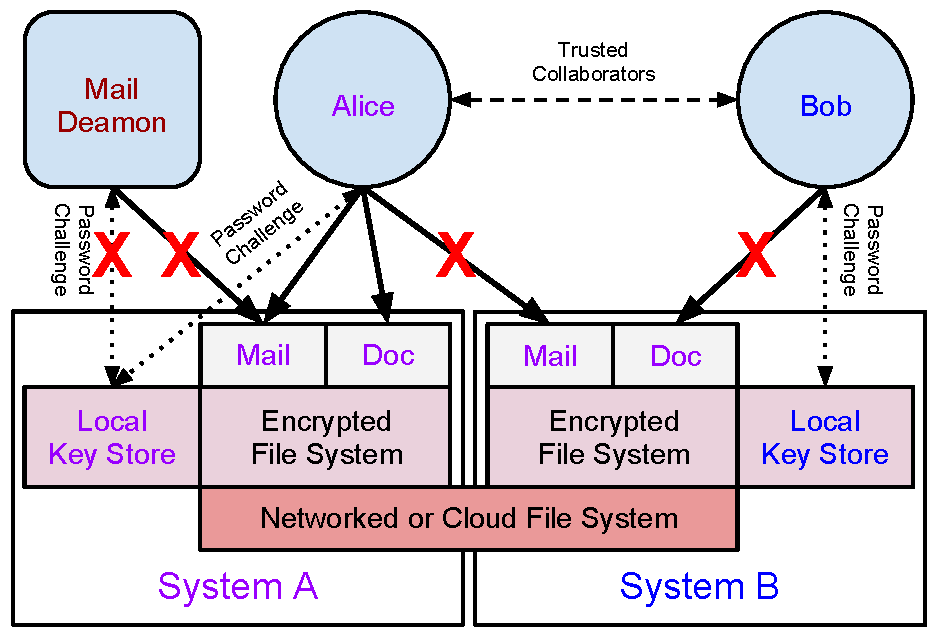
\includegraphics[width=\columnwidth]{./include/Problem-Layered.pdf}
  \caption{Existing Local Encrypted File Systems}
  \label{fig:problem-layered}
\end{figure}

Existing local encrypted file system solutions like
dm-crypt~\cite{dm-crypt} and eCryptfs~\cite{Halcrow} suffer from a
number of limitations related to their tightly-coupled local key
storage and access management components. As Figure
\ref{fig:problem-layered} shows, these systems work fine for an
individual user like Alice wishing to secure items like her mail or
documents and access them from a single machine. But they quickly
break down when trying to move beyond the simple single-user,
single-device use case. Alice can not access her encrypted mail file
across a networked file system from System B since System B has no
access to the encryption keys stored on System A. Furthermore, she can
not share a work document with a trusted collaborator like Bob, since
Bob neither has access to her encryption keys stored on System A nor
the password required to unlock these keys. A non-interactive process
like the Mail Daemon is also unable to leverage these encrypted file
systems due to the inability of such services to securely and
interactively provide a password to unlock the keys needed to decrypt
local files.

\begin{figure}[!tb]
  \centering
  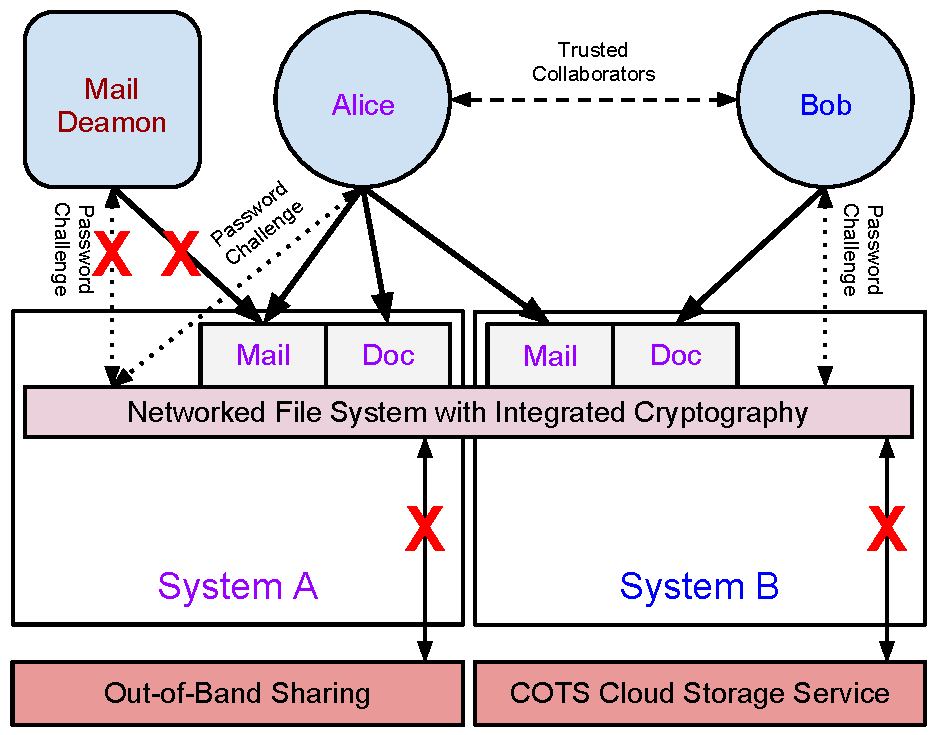
\includegraphics[width=\columnwidth]{./include/Problem-Integrated.pdf}
  \caption{Existing Distributed Encrypted File Systems}
  \label{fig:problem-integrated}
\end{figure}

While distributed encrypted file systems such as
OceanStore~\cite{Kubiatowicz2000}, Plutus~\cite{Kallahalla2003},
Cumulus4j~\cite{cumulus4j}, or Tahoe~\cite{Wilcox-O'Hearn2008} tend to
succeed in solving some of the sharing and distribution problems
inherent in local secure file systems, they still lack the flexibility
required to address the full range of desired use cases. Figure
\ref{fig:problem-integrated} shows some of the remaining issues
inherent in distributed solutions. Notably, while multi-user use cases
are better supported, non-interactive use cases are still a
challenge. Furthermore, full stack distributed file systems tend to be
wedded with specific storage systems and thus lack support for
Cloud-based Storage as a Service offerings or alternate underlying
storage technologies. These systems also lack support for most forms
of ``out-of-band'' file sharing (via e-mail, USB flash drives, etc)
due to the inability of actors outside of the integrated stack to
access the necessary encryption keys.

Existing systems force the user into a very specific security model,
appropriate for certain use cases, but useless for many others. These
systems also only support to a handful of technologies often excluding
alternate, new, or unforeseen options. They fail to accommodate our
natural usage patterns, and thus often go unused. The solution is to
acknowledge the fact that one-size-does-not-fit-all when it comes to
securing our data. And then to build a system around this principle,
capable of supporting an extensible range of use cases. Toward this
end we present Custos: a flexible ``Key Storage as a Service'' system
designed to support a variety of data security requirements across a
wide range of use cases. Custos is based on three core principles:

\begin{packed_item}
\item Decoupled Key Storage
\item Flexible Security Models
\item Global Access and Centralization
\end{packed_item}

We propose the following common use-case examples, none of which are
well supported by existing encryption systems, that we believe can be
better supported by using Custos-integrated encryption systems:

\begin{packed_desc}
\item[Secure Multi-Devices Access:] Alice uses Dropbox~\cite{dropbox} to
  synchronize her files between her work computer, her home computer,
  and her tablet. She wishes to encrypt her Dropbox-synced files
  while maintaining the ability to access and modify files across all
  of her devices regardless of the device on which they were created
  or originally encrypted.
\item[Secure Out-of-Band Sharing:] Alice wants to send Bob an
  encrypted file via e-mail attachment or USB flash drive. She wishes
  to grant Bob secure access to the file so that Bob and decrypt and
  read the file easily without requiring a cumbersome manual exchange
  of encryption keys via a phone call or in-person meeting.
\item[Secure Autonomous Access:] Alice has an account on a server
  where she uses a file-level encryption system like
  eCryptfs~\cite{eCryptfs} to encrypt her home directory,
  automatically decrypting her files when she is logged in. Alice has
  a mail forwarding configuration file in her home directory that
  directs the local mail server to forward e-mail sent to this server
  to her primary e-mail account. Thus, she must grant the local mail
  daemon autonomous access to that single encrypted configuration file
  while retaining the interactive log in requirement for access to all
  her other home directory files.
\end{packed_desc}

Through the remainder of the paper we will discuss Custos and how it's
flexibility can accommodate these, and many other, use-case
examples. In \S \ref{sec:principles} we discuss the core Custos
concepts in more depth. We go on to present the architectures of
Custos in \S \ref{sec:arch}. Finally, we close by discussing the
current state of the Custos project and our visions for the future in
\S \ref{sec:conclusion}.
